%%%%%%%%%%%%%%%%%%%%%%%%%%%%%%%%%%%%%%%%%
% Homework Assignment Article
% LaTeX Template
% Version 1.3.1 (ECL) (08/08/17)
%
% This template has been downloaded from:
% Overleaf
%
% Original author:
% Victor Zimmermann (zimmermann@cl.uni-heidelberg.de)
%
% License:
% CC BY-SA 4.0 (https://creativecommons.org/licenses/by-sa/4.0/)
%
%%%%%%%%%%%%%%%%%%%%%%%%%%%%%%%%%%%%%%%%%

%----------------------------------------------------------------------------------------

\documentclass[a4paper]{article} % Uses article class in A4 format

%----------------------------------------------------------------------------------------
%	FORMATTING
%----------------------------------------------------------------------------------------

\addtolength{\hoffset}{-2.25cm}
\addtolength{\textwidth}{4.5cm}
\addtolength{\voffset}{-3.25cm}
\addtolength{\textheight}{5cm}
\setlength{\parskip}{0pt}
\setlength{\parindent}{0in}

%----------------------------------------------------------------------------------------
%	PACKAGES AND OTHER DOCUMENT CONFIGURATIONS
%----------------------------------------------------------------------------------------

\usepackage{blindtext} % Package to generate dummy text
% \usepackage[style=numeric,sorting=none]{biblatex}
\usepackage{charter} % Use the Charter font
\usepackage[utf8]{inputenc} % Use UTF-8 encoding
\usepackage{microtype} % Slightly tweak font spacing for aesthetics

\usepackage[english]{babel} % Language hyphenation and typographical rules

\usepackage{amsthm, amsmath, amssymb} % Mathematical typesetting
\usepackage{float} % Improved interface for floating objects
\usepackage[final, colorlinks = true, 
            linkcolor = black, 
            citecolor = black]{hyperref} % For hyperlinks in the PDF
\usepackage{graphicx, multicol} % Enhanced support for graphics
\usepackage{xcolor} % Driver-independent color extensions
\usepackage{marvosym, wasysym} % More symbols
\usepackage{rotating} % Rotation tools
\usepackage{censor} % Facilities for controlling restricted text
\usepackage{listings, style/lstlisting} % Environment for non-formatted code, !uses style file!
\usepackage{color}

\definecolor{dkgreen}{rgb}{0,0.6,0}
\definecolor{gray}{rgb}{0.5,0.5,0.5}
\definecolor{mauve}{rgb}{0.58,0,0.82}
\lstset{frame=tb,
  language=Java,
  aboveskip=3mm,
  belowskip=3mm,
  showstringspaces=false,
  columns=flexible,
  basicstyle={\small\ttfamily},
  numbers=none,
  numberstyle=\tiny\color{gray},
  keywordstyle=\color{blue},
  commentstyle=\color{dkgreen},
  stringstyle=\color{mauve},
  breaklines=true,
  breakatwhitespace=true,
  tabsize=3
}
\usepackage{pseudocode} % Environment for specifying algorithms in a natural way
\usepackage{style/avm} % Environment for f-structures, !uses style file!
\usepackage{booktabs} % Enhances quality of tables

\usepackage{tikz-qtree} % Easy tree drawing tool
\tikzset{every tree node/.style={align=center,anchor=north},
         level distance=2cm} % Configuration for q-trees
\usepackage{style/btree} % Configuration for b-trees and b+-trees, !uses style file!

% \usepackage[backend=biber,style=numeric,
            % sorting=nyt]{biblatex} % Complete reimplementation of bibliographic facilities
% \addbibresource{ecl.bib}
\usepackage{csquotes} % Context sensitive quotation facilities

\usepackage[yyyymmdd]{datetime} % Uses YEAR-MONTH-DAY format for dates
\renewcommand{\dateseparator}{-} % Sets dateseparator to '-'

\usepackage{fancyhdr} % Headers and footers
\pagestyle{fancy} % All pages have headers and footers
\fancyhead{}\renewcommand{\headrulewidth}{0pt} % Blank out the default header
\fancyfoot[L]{School of Computing, Macquarie University} % Custom footer text
\fancyfoot[C]{} % Custom footer text
\fancyfoot[R]{\thepage} % Custom footer text

\usepackage{comment}
\newcommand{\note}[1]{\marginpar{\scriptsize \textcolor{red}{#1}}} % Enables comments in red on margin

\hypersetup{
    colorlinks=true,
    linkcolor=blue,
    filecolor=magenta,      
    urlcolor=cyan,
    pdftitle={COMP3100 Assignment 1},
    pdfpagemode=FullScreen,
    }

%----------------------------------------------------------------------------------------

\begin{document}

%----------------------------------------------------------------------------------------
%	TITLE SECTION
%----------------------------------------------------------------------------------------

\title{COMP3100 project report} % Article title
\fancyhead[C]{}
\hrule \medskip % Upper rule
\begin{minipage}{1\textwidth} % Center of title section
\centering 
\large % Title text size
Project report: Stage 1\\ % Assignment title and number
COMP3100 Distributed Systems, S2, 2022\\
\normalsize % Subtitle text size
SID: 41478886, Name: James Nugent
%%%%\\ % Assignment subtitle
\end{minipage}
\medskip\hrule % Lower rule
\bigskip

%----------------------------------------------------------------------------------------
%	ARTICLE CONTENTS
%----------------------------------------------------------------------------------------

\section*{Introduction}
The first assignment for COMP3100 involves creating a scheduler to operate in tandem with the ds-sim server application.
The scheduler would assign jobs using a naive `round robin' algorithm, only allocating to the servers within the largest type as defined by the number of cores each server has.
The purpose of the assignment was to introduce students to some concepts in distributed systems such as job scheduling, as well as some core java programming concepts such as socket programming.
This report outlines the development of a suitable client with the Largest Round Robin (LRR) algorithm implemented, including the system overview, design and implementation.

\section*{System Overview}

The job scheduling system as outline by the ds-sim project \cite{dssim} contains two separate processes; the ds-server, and client.
The ds-server handles the system information, system state, and event generation.
Events can include job completions, job requests, job and machine failures as well as machine recoveries.
The ds-server generates events either based on a config file passed in at startup or are randomly generated. A seed can also be used to allow for repeat executions with the same state and events. The server will push these events to a client, and will wait until the client responds before it generated the next event.
\newline
The client will initially connect to the server using a handshake then indicate that it is ready to process the first event.
The client should send a message back to the server if it wishes to schedule/push/move/cancel a job, query the server state, or inform the server it's ready for the next message.
The messaging between the two processes occurs over a TCP socket. This means that the server and client can reside on different machines if that is required during simulation.
Another way the server can interact with the client is that the ds-server will write a ds-system.xml file after handshaking with the client.
The client can read this file in to the get information on the available machines within the simulated system.
This however is only a one-way communication channel as the ds-server will not consume any files from the file-system.
A simplified diagram of the system can be seen in figure \ref{ds-sim_overview}
\begin{figure}[H]
    \centering
    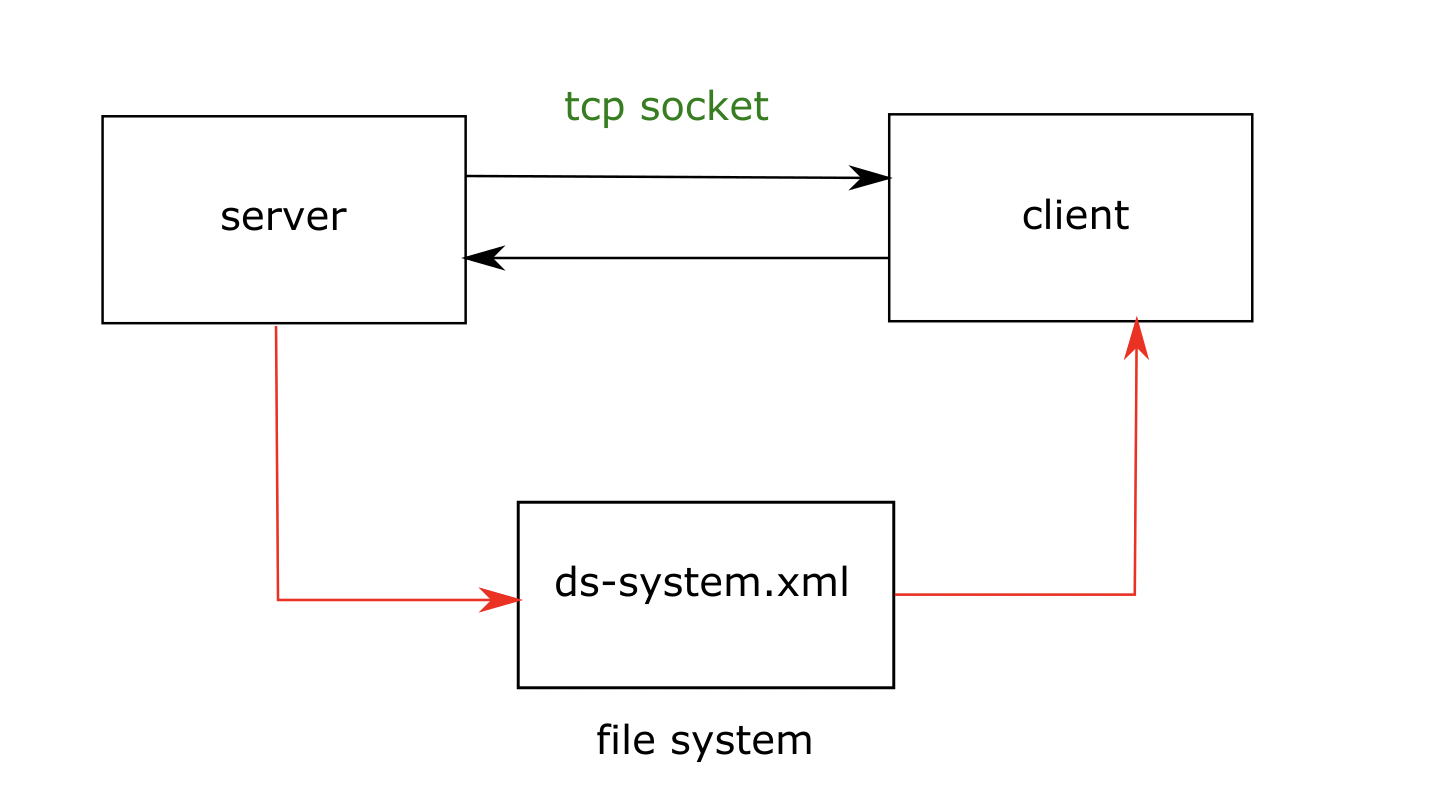
\includegraphics[scale=0.5]{./ds-sim_architecture.png}
    \caption{Simple DS-Sim System Overview}
    \label{ds-sim_overview}
\end{figure}


\section*{Design}
The client for this was designed so that the algorithm for scheduling is separate from the running of the scheduler. The messaging to the server was also abstracted into a service to remove unnecessary implementation details from the scheduler and algorithm.
This decision was made so that the algorithm can be considered to be a simple state machine that will run until it arrives at a final state. 
With this in mind the client can be considered, at a high level, three separate parts; the scheduler, algorithm, and the messaging service.
A note on the verbage used: scheduler is a bit of a misnomer, as the scheduler itself cannot run without an algorithm. The scheduler is really the term used for the code that executes an algorithm until it's final state or an error.
\\
\\
For the scheduler to run it requires 2 components or arguments, a state machine function and an initial state. 
A state machine function is defined as a function over the incoming message from ds-server and the current state.
It then returns the new state. The scheduler then reads in the new message from the server and invokes the function again with the new state.
This occurs until a state is return that is consider 'finished'. 
\subsection*{Scheduling Algorithms}
To make the implementation of algorithms as simple as possible and algorithm only needs to provide 2 things to be run by the scheduler, a transition function, and an initial state.
The transition function essentially forms a state action or state transition \cite{scala_fp} over a specified 'state type', which contains all the information the algorithm needs to schedule jobs.
While not in the scope of this project one example of that would be a list of the unavailable/failed servers, so the algorithms could make sure they don't assign jobs to servers that will not process them.
Another advantage of using a functional programming paradigm is that the state transitions can be built individually and the used in combinators \cite{scala_fp}.
The state object can be as simple or complex as needed by the algorithm, but must fulfill the 'State' algorithm provided, which has a single getter. The getter function fetches a boolean that determines whether or not the algorithm has finished running.
\subsubsection*{Last Round Robin}
The last round robin algorithm is a naive algorithm that simply assigns jobs to the servers with the most CPU's.
In the event of a tie between server types the first found server type is used and only machines in that server type are used.
The machine types are read in from the ds-system.xml as to not burden the ds-server with calls too regularly.
Once the largest machine type is determined the ds-server is queried for the number of servers. 
As each job request message comes in from the ds-server the algorithm will try to assign the job to the "next available server".
Once the algorithm reaches the last machine in the server type, it simply restarts the process from the first machine.
This loop continues until there are no more jobs to assign.

\section*{Implementation}
The implementation of the described design used both object oriented paradigms, as well as functional programming paradigms.
The combination of the two would allow for a software package that allows for more algorithms to be implemented with great ease, with many objects abstracting technical details away allowing the programmer interact with the business-logic of the ds-sim system.
\subsection*{Socket Communication}
The first level of abstraction that exists in the solution is the abstraction of the socket messaging. 
The client interacts with the ds-server using sockets, but the operation of the algorithm and scheduling does not need to know about the specifics of that interaction.
\newline
Because of this we abstract the reading and writing of the messages over the socket into two separate functions that return a string, or consume (send) a string.
There are two notable things about this abstraction. The first is the use of anonymous functions.
The anonymous function allows us to reduce the amount of code needed to abstract the socket interaction away from the messaging service (which comes later). 
The second is the use of the Either class. An Either allows us to handle exceptions in a more functional way\cite{bly_2018}.
The either class has two states, left and right and they represent the result of some computation (or function call). 
Standard practice is that the 'left' value represents the error, while the 'right' value represents the result of the computation.
An either cannot be both 'left' and 'right'. Using this we can handle errors without dealing with exceptions, which can often be costly in computation time \cite{maurer_2013}. 
One way to think of an either in Java terms is that it is essentially a function that throws an exception, with the exception mapping to the 'left' value and the return value mapping to the 'right'.
Using this class we can code freely without having to deal with the exceptions from dealing with the Socket class, and just worry about mapping the read or written value.

\subsection*{Client Messaging System}
Given that we now have a generic function for read and a generic function for writing we can now build a service that will allow us to abstract some ds-server implementation details out from the rest of the system.
We abstract the interactions with the ds-server into the follow functions:
\begin{itemize}
    \item signalRedy
    \item getServerState
    \item loginToServer
    \item scheduleJob
    \item quit
    \item pushJob
    \item getMessage
    \item beginScheduling
\end{itemize}
loginToServer takes a string, username, and performs the required handshaking to start the server.
Scheduling a job is handled by the scheduleJob function (because of course it should \cite{loureiro_2015}). It simply takes the job id, server type and server id, then constructs the schedule message then sends it.
The quit function handles the final handshake required to complete the simulation. It also runs a 'finish' function that is provided on construction to the CMS in case there is anything needed to be done by the CMS implementation (for example, closing sockets).
`pushJob' is simply a wrapper around sending the 'PSHJ' message. The `beginScheduling' function is simply a rename of the `signalRedy' function, but was extracting in case there were other operations required to start the scheduling, compared to signaling to the ds-server that the client is ready for the next message. A future piece of refactor work could be to remove this as it's current redundant. 
\newline
The 'getServerState' function send the GETS message to the server based on the ConfigRequest pojo.
This pojo represents the params of the GETS message, and can also be deserialized to the proper format to be send to the ds-server.
The function then returns a list of the ServerStateItem pojos, which represent the various machines in the system. This pojo is based on the XSD for the ds-system.xml file.
The function is also overloaded so it can be called with no request arg to retrieve the entire system configuration, which corresponds to the 'GETS All' call.
Other abstractions could be put into the service, but none were necessary to implement the LRR algorithm.
\subsection*{LRR Algorithm Implementation}
Since the ClientMessagingService (CMS) gives us a way to interface with the ds-server on a purely business logic level, we can now easily implement a state action for our algorithm.
First we define a state object. For the LRR algorithm there are only 3 pieces of information we need to keep track off (outside of whether or not the state is a finishing state):
\begin{itemize}
    \item The largest server type
    \item The id of the last server a job was scheduled to
    \item The total number of machines with the largest server type
\end{itemize}
This state definition depends on some nuance of the ds-server, in that all server ids are based on an integer sequence that increases by 1. 
If the machine ids were not a monotonically increasing sequence the state would have to capture a list of ids that defined the order in which the jobs would be scheduled.
Since the largest server type, and total number of machines should never change once the system is running, a piece of future work could be to create a state that is simpler and create a closure over those two variables instead of carrying them around in the state pojo.
\newline
With that state definition we can create a simple state action that will be invoked each time a new message is received. 
The easiest way to define that state action is by thinking of the operations for each received message. The most complicated of these will be the JOBN message, which corresponds to the ds-server generating a job to be scheduled.
For this message the state action will get id of the next server to have a job scheduled. This is a simple mathematical formula 
\begin{math}
    x = (y + 1) \bmod n
\end{math}
where y is the id of the server that was last assigned a job, and n is the number of servers with the largest server type.
The function then uses the CMS to schedule the job and tells the ds-server it is ready for the next message.
It generates the new state and returns it.
\newline
The other parts of the state action are much simpler. If we receive the 'NONE' message we return a new state that is marked as finished.
All other messages will end up returning the same state as before, except the processing for a job completed message will also indicate to the ds-server that we're ready to receive the next message.
\subsection*{Scheduling Service}
With the definition of a state action and state object defined we can now delve into the implementation of the scheduling service.
The scheduling service should not care for the specific details of the LRR algorithm, but rather the generic description of the state action and state definition. 
The service should also be able to map the algorithms to some key so that we can store and run different types of algorithms that can be driven by command-line arguments.
The easiest way to store this would be to take a map of the state actions and an initial state.
However, to keep the algorithms as pure functions and to take advantage of the anonymous functions in Java 8 we need some way to pass in the CMS to the state action. 
The easiest way to do this is to use the factory pattern. The factory pattern is based on the idea of separating the creation of an object from it's definition \cite{gamma_2016}.
While the definition of our factory is closer to a closure than a traditional factory the ideal of the pattern still remains.
We can also see that the definition returns the initial state meaning that an 'algorithm' actuall consists of the state action and the initial state.
\newline
\begin{figure}[ht!]
\label{algorithm_factory}
\begin{lstlisting}
@FunctionalInterface
public interface AlgorithmFactory<T extends State> {
    Pair<StateMachine<T, String>, Either<String, T>> createAlgorithm(ClientMessagingService cms);
}
\end{lstlisting}
\caption{Definition of our algorithm factory interface}
\end{figure}
The scheduling service can now take a map of algorithm factories so it can run many different algorithms.
However, due to the way generics work in Java 8 the map definition erases the generic type of 'T', and assumes that all algorithms are of type \lstinline{? extends State}\ref{ss_ctor}.
\begin{figure}[ht!]
\begin{lstlisting}
public SchedulingService(final ClientMessagingService clientMessagingService, Map<String, Pair<StateMachineFactory<? extends State>, StateConfigurationFactory<? extends State>>> algorithms) {
    this.clientMessagingService = clientMessagingService;
    this.algorithms = algorithms;
}
\end{lstlisting}
\label{ss_ctor}
\caption{Constructor definition for the Scheduling Service}
\end{figure}
\newline
With a map of algorithms that the service can run we look at the definition of the main function that will run the algorithm to completion.
The running of the algorithm is covered by two functions: `scheduleJobUsingAlgorithm`, and `run`.
The scheduleJobUsingAlgorithm function handles the handshaking to start the simulation, selects the algorithm to run by calling the factory to get the state action and initial state.
It then passes the action and state to the run function.
\newline

\begin{figure}[ht!]
\begin{lstlisting}
Either<String, String> run(StateMachine<State, String> stateMachine, State state, String initialMessage) {
        State currentState = state;
        Either<String, String> message = getNextMessage();
        while(true) {
            if (message.isLeft()) {
                return message; // Could not read message
            } else {
                Either<String, ? extends State> accept = stateMachine(message, state); // Run the state action
                if (accept.isLeft()) {
                    fail; //failed to process message
                } else {
                    currentState = accept.right().value();
                    if (currentState = finished) { 
                        finishRunningAlgorithm; // We finished processing
                    }
                }
            }
            message = clientMessagingService.getMessage(); // Get the next message and continue processing
        }
}
\end{lstlisting}
\label{run_psuedocode}
\caption{The psuedocode of the scheduling services run function}
\end{figure}
The run function is essentially a while loop that will continue processing messages until it gets a failure or the state machine returns a finished state. 
Between the scheduling function that handshakes, and the run function that performs the actual state transforms that covers the entirety of the implementation of the SchedulingService.
\subsection*{Test Driven Development}
While most of the implementation fell out of the design of the system the actual implementation was achieved by using Tes Driven Development (TDD).
TDD is the practice of writing tests first, then the code needed to verify those tests \cite{beck_2015}.
This practice allows for more robust code, and when partnered with git made it easy to roll-back bugs if they cropped up. 
Whilst this might be an unnecessary practice for a solo project, it definitely helped when refactoring large chunks of the code base.
One example was when moving from using a class to define the algorithm factory to using anonymous functions. 
Because there were many tests ensuring the quality of the code, and the fact a common interface was coded to I could make changes to the implementation without wondering whether it works or not.
\section*{Conclusion}
The design and implementation presented in this report shows a robust, extensible, and well-tested client to interact with the ds-sim server. 
The implementation also shows a firm understanding of object oriented programming, functional programming, as well as test driven development.
While it may seem counter-intuitive to implement function programming techniques in an OO language, the use of pure functions allows for a far more testable and cleaner algorithm implementation.


\subsection*{Code Repositories}
\begin{itemize}
    \item \hyperlink{https://github.com/jamesnuge/comp3100-assignment1}{Github repository}
    \item \hyperlink{https://bitbucket.org/jamesnuge/assignment-1}{Bitbucket repository}
\end{itemize}

%----------------------------------------------------------------------------------------
%	REFERENCE LIST
%----------------------------------------------------------------------------------------
\bibliographystyle{ieeetr}
\bibliography{comp3100project}
% \printbibliography

%----------------------------------------------------------------------------------------

\end{document}
